\documentclass[12pt,a4paper,twoside]{report}

\usepackage[utf8]{inputenc}
\usepackage{graphicx}
\graphicspath{ {figures/} }
\usepackage{pgfplots}                %% for ploting in latex
\usepgfplotslibrary{external}
\usetikzlibrary{pgfplots.groupplots} %% pgf groupplots
%\usetikzlibrary{pgfplots.external}
%\tikzexternalize
\usepackage{caption}
\usepackage{subcaption}
\usepackage{xcolor,cancel}
\usepackage{adjustbox}  %% e.g. wrap verbatim larger than linewidth
\usepackage{fancyvrb}   %% Verbatim and coloring therein
\usepackage{hyperref}
\usepackage{imakeidx}   %% for index
\makeindex[columns=3, title=Alphabetical Index]
\usepackage{soul}       %% allow wrapping of underlined text, via \ul{...}
\usepackage{natbib}     %% for bibliography
%\usepackage[left=2cm,right=2cm]{geometry} % somewhat wider text to allow code
\usepackage{geometry}   %% somewhat wider text to allow code
\usepackage[per-mode=symbol]{siunitx}    %% SI Units
\usepackage{amsmath,amssymb,amsthm,bm} %% for math ...
\usepackage{mathabx}
\usepackage{mathtools}
\usepackage[most]{tcolorbox} %% colorboxes for equations
\usepackage[acronym, toc, nonumberlist]{glossaries} %% for acronyms
\usepackage{tabularx}
\usepackage{multirow}  %% for tabular
\usepackage{todonotes} %% fancy, right-margin notes
\usepackage{csquotes}  %% for quoting
\usepackage{wasysym}   %% zodiac symbols (equinox, etc ...)
\usepackage{algorithm2e} %% for pseudocode/algorithms
\usepackage{footmisc} %% for referencing footnotes (provides \footref)

%% TikZ stuff %%
\usepackage{tikz} % add a few drawings ...
\usepackage{tkz-euclide}
\usepackage{tikz-3dplot}
\usetikzlibrary{matrix}
\usetikzlibrary{shapes.geometric, arrows} % for creating tikz flowcharts 
\usetikzlibrary{shapes.misc}
\usetikzlibrary{calc}
\usetikzlibrary{quotes,angles}
\usetikzlibrary{positioning}
\usetikzlibrary{mindmap,trees}

\usepackage{listings} % include source code files
% Solarized colour scheme for listings
\definecolor{solarized@base03}{HTML}{002B36}
\definecolor{solarized@base02}{HTML}{073642}
\definecolor{solarized@base01}{HTML}{586e75}
\definecolor{solarized@base00}{HTML}{657b83}
\definecolor{solarized@base0}{HTML}{839496}
\definecolor{solarized@base1}{HTML}{93a1a1}
\definecolor{solarized@base2}{HTML}{EEE8D5}
\definecolor{solarized@base3}{HTML}{FDF6E3}
\definecolor{solarized@yellow}{HTML}{B58900}
\definecolor{solarized@orange}{HTML}{CB4B16}
\definecolor{solarized@red}{HTML}{DC322F}
\definecolor{solarized@magenta}{HTML}{D33682}
\definecolor{solarized@violet}{HTML}{6C71C4}
\definecolor{solarized@blue}{HTML}{268BD2}
\definecolor{solarized@cyan}{HTML}{2AA198}
\definecolor{solarized@green}{HTML}{859900}

% Define C++ syntax highlighting colour scheme
\lstset{language=C++,
        basicstyle=\footnotesize\ttfamily,
        numbers=left,
        numberstyle=\tiny,
        tabsize=2,
        breaklines=true,
        escapeinside={@}{@},
        numberstyle=\tiny\color{solarized@base01},
        keywordstyle=\color{solarized@green},
        stringstyle=\color{solarized@cyan}\ttfamily,
        identifierstyle=\color{solarized@blue},
        commentstyle=\color{solarized@base01},
        emphstyle=\color{solarized@red},
        frame=single,
        rulecolor=\color{solarized@base2},
        rulesepcolor=\color{solarized@base2},
        showstringspaces=false
}

% include the external source file, instead of pasting its contents directly 
% into the LaTeX documen
\newcommand{\codelst}[1]{\lstinputlisting[caption=\texttt{\protect\detokenize{#1}}]{#1}\newpage}

% a macro to write norms
\newcommand\norm[1]{\lVert#1\rVert}
% a macro to write derivative at:
% examples: 1. $f'(x)\at{x=1}$
%           2. $f'(x)\at[\big]{x=1}$
\newcommand{\at}[2][]{#1|_{#2}}
% Symbols for Love numbers, h, k, and l
\newcommand{\lovek}{k}
\newcommand{\loveh}{h}
\newcommand{\lovel}{l}
% Imaginary i
\newcommand{\iim}{{i\mkern1mu}}

% dBm unit
\DeclareSIUnit{\belmilliwatt}{Bm}
\DeclareSIUnit{\dBm}{\deci\belmilliwatt}
\DeclareSIUnit{\cycles}{cycles}
\DeclareSIUnit\century{century}
\DeclareSIUnit\year{yr}
\DeclareSIUnit\larcsecond{as} %% literal arcsecond

% augment the paragraph skip ... a bit more clear text
\setlength{\parskip}{1em}

% equation colorbox
\tcbset{colback=yellow!5!white, colframe=red!50!black,
        highlight math style= {enhanced, %<-- needed for the ’remember’ options
            colframe=red,colback=red!10!white,boxsep=0pt}
        }

% mathmode strikethrough command, see
% https://tex.stackexchange.com/questions/20609/strikeout-in-math-mode#20613
\newcommand\hcancel[2][black]{\setbox0=\hbox{$#2$}%
\rlap{\raisebox{.45\ht0}{\textcolor{#1}{\rule{\wd0}{1pt}}}}#2}

\bibliographystyle{plainnat}

\makeglossaries
\newacronym{ids}{IDS}{International DORIS Service}
\newacronym{antex}{ANTEX}{Antenna Exchange Format}
\newacronym{pcv}{PCV}{Phase Center Variations}
\newacronym{pco}{PCO}{Phase Center Offset}
\newacronym{iers}{IERS}{International Earth Rotation and Reference Systems Service}
\newacronym{era}{ERA}{Earth Rotation Angle}
\newacronym{gst}{GST}{Greenwich Sidereal Time}
\newacronym{tio}{TIO}{Terrestrial Intermediate Origin}
\newacronym{vlbi}{VLBI}{Very Long Baseline Interferometry}
\newacronym{ode}{ODE}{Ordinary Differential Equation}
\newacronym{rkn}{RKN}{Runge-Kutta-Nystr{\"o}m}
\newacronym{snc}{SNC}{State Noise Compensation}
\newacronym{dmc}{DMC}{Dynamic Model Compensation}
\newacronym{icrf}{ICRF}{International Celestial Reference Frame}
\newacronym{icrs}{ICRS}{International Celestial Reference System}
\newacronym{crs}{CRS}{Celestial Reference System}
\newacronym{gcrf}{GCRF}{Geocentric Celestial Reference Frame}
\newacronym{gcrs}{GCRS}{Geocentric Celestial Reference System}
\newacronym{bcrf}{BCRF}{Barycentric Celestial Reference Frame}
\newacronym{bcrs}{BCRS}{Barycentric Celestial Reference System}
\newacronym{cip}{CIP}{Celestial Intermediate Pole}
\newacronym{cio}{CIO}{Celestial Intermediate Origin}
\newacronym{iau}{IAU}{International Astronomical Union}
\newacronym{cirs}{CIRS}{Celestial Intermediate Reference System}
\newacronym{itrs}{ITRS}{International Terrestrial Reference System}
\newacronym{tirs}{TIRS}{Terrestrial Intermediate Reference System}
\newacronym{itrf}{ITRF}{International Terrestrial Reference Frame}
\newacronym{irf}{IRF}{Inertial Reference Frame}
\newacronym{trf}{TRF}{Terrestrial Reference Frame}
\newacronym{tcb}{TCB}{Barycentric Coordinate Time}
\newacronym{tcg}{TCG}{Geocentric Coordinate Time}
\newacronym{tt}{TT}{Terestrial Time}
\newacronym{tai}{TAI}{International Atomic Time}
\newacronym{eop}{EOP}{Earth Orientation Parameters}
\newacronym{erp}{ERP}{Earth Rotation Parameters}
\newacronym{leo}{LEO}{Low Earth Orbit}
\newacronym{sinex}{SINEX}{Solution INdependent EXchange Format}
\newacronym{cnes}{CNES}{Centre National d'Etudes Spatiales (National Centre for Space Studies)}
\newacronym{catr}{CATR}{Compact Antenna Test Range}
\newacronym{utc}{UTC}{Coordinated Universal Time}
\newacronym{sofa}{SOFA}{Standards Of Fundamental Astronomy}
\newacronym{fcn}{FCN}{Free Core Nutation}
\newacronym{ut1}{UT1}{Universal Time}
\newacronym{tgp}{TGP}{Tide Generating Potential}
%\newacronym{}{}{}


\title{\texttt{libgeodesy} Manual}
\author{Xanthos}
\date{\today}

\begin{document}

\begin{titlepage}
\maketitle
\end{titlepage}

%\frontmatter
\tableofcontents
\listoffigures
\listoftables

\chapter{Ellipsoidal Geometry}
\label{ch:ellipsoidal-geometry}

\subsection{Ellipsoid}
\label{sec:ellipsoid}
The shape of the ellipsoid is described by two geometric parameters, the 
\emph{semi-major} axis $\alpha$ and the \emph{semi-minor} axis $b$. $b$ is 
often replaced by the \emph{flattening} $f$, a smaller quantity describing the 
small polar flattening of the ellipsoid. $f$ is given by the formula:
\begin{equation}
  f = \frac{\alpha -b}{b}
  \label{eq:flattening}
\end{equation}

\subsubsection{Eccentricity}
\label{sssec:eccentricity}
The eccentricity can be expressed as:
\begin{equation}
  e = \sqrt{1 - \left( \frac{b}{a} \right)^2 }
    = \frac{\sqrt{\alpha ^2 - b^2}}{\alpha}
  \label{eq:eccentricity-1}
\end{equation}

Note that from \ref{eq:eccentricity-1}, we have:
\begin{equation}
  \sqrt{1-e^2} = \frac{b}{\alpha} = 1 - f
  \label{eq:eccentricity-2}
\end{equation}

\subsubsection{Ellipsoidal, Geocentric and Reduced Latitude}
\label{sssec:ellipsoidal-and-geocentric-latitude}

\begin{figure}
  \centering
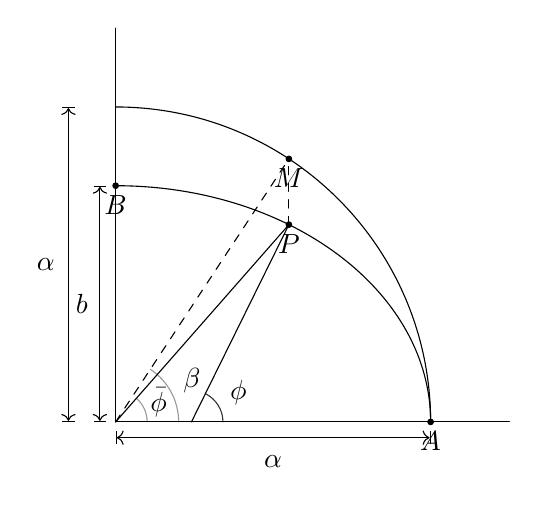
\begin{tikzpicture}[line cap=round,line join=round]
  \pgfmathsetmacro{\rc}{4}
  \pgfmathsetmacro{\rb}{3.0}
  \pgfmathsetmacro{\xp}{2.2}
  \pgfmathsetmacro{\yp}{\rb * sqrt((1-(\xp * \xp)/(\rc *\rc))}
  \pgfmathsetmacro{\ecsq}{(\rc*\rc -\rb *\rb)/(\rc *\rc)}
  \tkzDefPoint(0,0){C}
  \tkzDefPoint(\rc,0){A}
  \tkzDefPoint(0,\rb){B}
  \tkzDefPoint(5,0){X}
  \tkzDefPoint(0,5){Y}
  \tkzDefPoint(\xp,\yp){P}
  \draw[name path=CX] (C)--(X);
  \draw[name path=CY] (C)--(Y);
  %\draw[name intersections={of=elip and AC, by={D}}];
  \tkzDrawPoints[fill=black](A,B,P)
  \tkzLabelPoints(A,B,P)
  \tkzFindAngle (A,C,B) \tkzGetAngle{an} \FPround\an\an{0} % 90 deg
  \pgfmathsetmacro{\ann}{atan2(sin(\an),cos(\an)/3)}
  \draw (A) arc (0:\ann:\rc cm and \rb cm);
  \draw (A) arc (0:\ann:\rc cm and \rc cm);
  \draw[name path=CP] (C)--(P); % geocentric
  \tkzMarkAngle[fill=yellow,
    size=0.4,
    opacity=0.4](A,C,P)
  \tkzLabelAngle[pos=.6](A,C,P){$\bar{\phi}$}
  \pgfmathsetmacro{\xpn}{\xp * \ecsq}
  \tkzDefPoint(\xpn,0){N}
  \draw[name path=NP] (N)--(P);
  \tkzMarkAngle[fill=red,
    size=0.4,
    opacity=0.8](A,N,P)
  \tkzLabelAngle[pos=.7](A,N,P){$\phi$}
  \pgfmathsetmacro{\ypc}{sqrt(\rc *\rc - \xp *\xp)}
  \tkzDefPoint(\xp,\ypc){M}
  \tkzDrawPoints[fill=black](M)
  \tkzLabelPoints(M)
  \draw[dashed, name path=PM] (P)--(M);
  \draw[dashed, name path=CM] (C)--(M);
  \tkzMarkAngle[fill=red,
    size=0.8,
    opacity=0.4](A,C,M)
  \tkzLabelAngle[pos=1.1](A,C,M){$\beta$}
  \draw [|<->|] ($(C)-(0,.2)$) -- node[below=1mm] {$\alpha$} ($(A)-(0,.2)$);
  \draw [|<->|] ($(C)-(.2,0)$) -- node[left=.3mm] {$b$} ($(B)-(.2,0)$);
  \tkzDefPoint(0,\rc){CB}
  \draw [|<->|] ($(C)-(.6,0)$) -- node[left=.5mm] {$\alpha$} ($(CB)-(.6,0)$);
\end{tikzpicture}
\caption{Ellipsoidal $\phi$, reduced $\beta$ and geocentric $\bar{\phi}$ latitude.}
\label{fig:latitudes}
\end{figure}

The \emph{geocentric} latitude $\bar{\phi}$, is related to the \emph{ellipsoidal} 
latitude $\phi$ (see \ref{fig:latitudes}) by the equation (\cite{Torge2001}, 
Section 4.1.1):
\begin{equation}
  \tan \bar{\phi} = \left( \frac{b}{\alpha} \right)^2 \tan \phi 
    = \left( 1 - e^2 \right) \tan \phi
\end{equation}

In \ref{fig:latitudes}, if we project (parallel to the $y$-axis) from point $P$ 
to the intersection of the coecentric circle (of radius $\alpha$), the geocentric 
angle obtained is labeled the \emph{reduced} latitude $\beta$. Reduced latitude 
can be expressed as a function of ellipsoidal latitude as (\cite{Torge2001}, 
Section 4.1.1):
\begin{equation}
  \tan \beta = \frac{b}{\alpha} \tan \phi = \sqrt{1-e^2} \tan \phi
  \label{eq:reduced-latitude}
\end{equation}

\begin{figure}
  \centering
  %\includegraphics[width=.65\linewidth, angle=-90]{Cryosat-2-RinexRfo}
  \includegraphics[width=.85\linewidth]{latitudes}
  \caption{Differences between ellipsoidal $\phi$, reduced $\beta$ and geocentric $\bar{\phi}$ latitude.}
  \label{fig:latitude-diffs}
\end{figure}



\bibliography{geodesy}

\glsaddall
\printglossary[type=\acronymtype,title=Acronyms]

\printindex

\end{document}
